\section{Giới thiệu nghiên cứu}

\subsection{Giới thiệu}

\indent Hiện nay các giải pháp công nghệ internet kết nối vạn vật - IoT đã và đang được nghiên cứu và triển khai rộng rãi, hướng tới kết nối toàn diện các thiết bị thông minh qua internet. Các ứng dụng IoT đang ngày càng phổ biến và xuất hiện thường xuyên ở cả những hoạt động hàng ngày của người dân. Đây là là tiền đề cho sự ra đời của nhà thông minh - Smarthome, kết hợp trí tuệ nhân tạo AI vào quản lý và vận hành nhà ở để hướng tới sự tiện nghi, chăm sóc sức khỏe, an ninh, an toàn và tiết kiệm năng lượng cho người dùng.

\indent Các hệ thống trong ngôi nhà thông minh nhờ đó không còn là thứ xa xỉ mà dần phổ biến với ưu điểm về tính kết nối và dễ sử dụng. Các thiết bị trong nhà thông minh đang bắt đầu giao tiếp với nhau, hoạt động như một nhóm thay vì các thiết bị riêng lẻ. Tính tiện lợi của nhà thông minh thể hiện qua khả năng cho phép người sử dụng điều khiển và sử dụng ngôi nhà mà không cần phải hiểu biết nhiều về công nghệ.

\indent Với khả năng tự động hóa và tích hợp công nghệ cao, nhà thông minh ngày càng trở thành một phần quan trọng của cuộc sống hiện đại. Tuy nhiên, để tối ưu hóa trải nghiệm người dùng, việc tìm kiếm phương pháp mới và hiệu quả để tương tác với hệ thống là hết sức quan trọng. Trong ngữ cảnh này, nghiên cứu này đặt ra vấn đề làm thế nào chúng ta có thể điều khiển các thiết bị trong Smart Home bằng cử chỉ tự nhiên của bàn tay, sử dụng kỹ thuật học máy và flex sensors.

\begin{figure}[H]
    \centering
    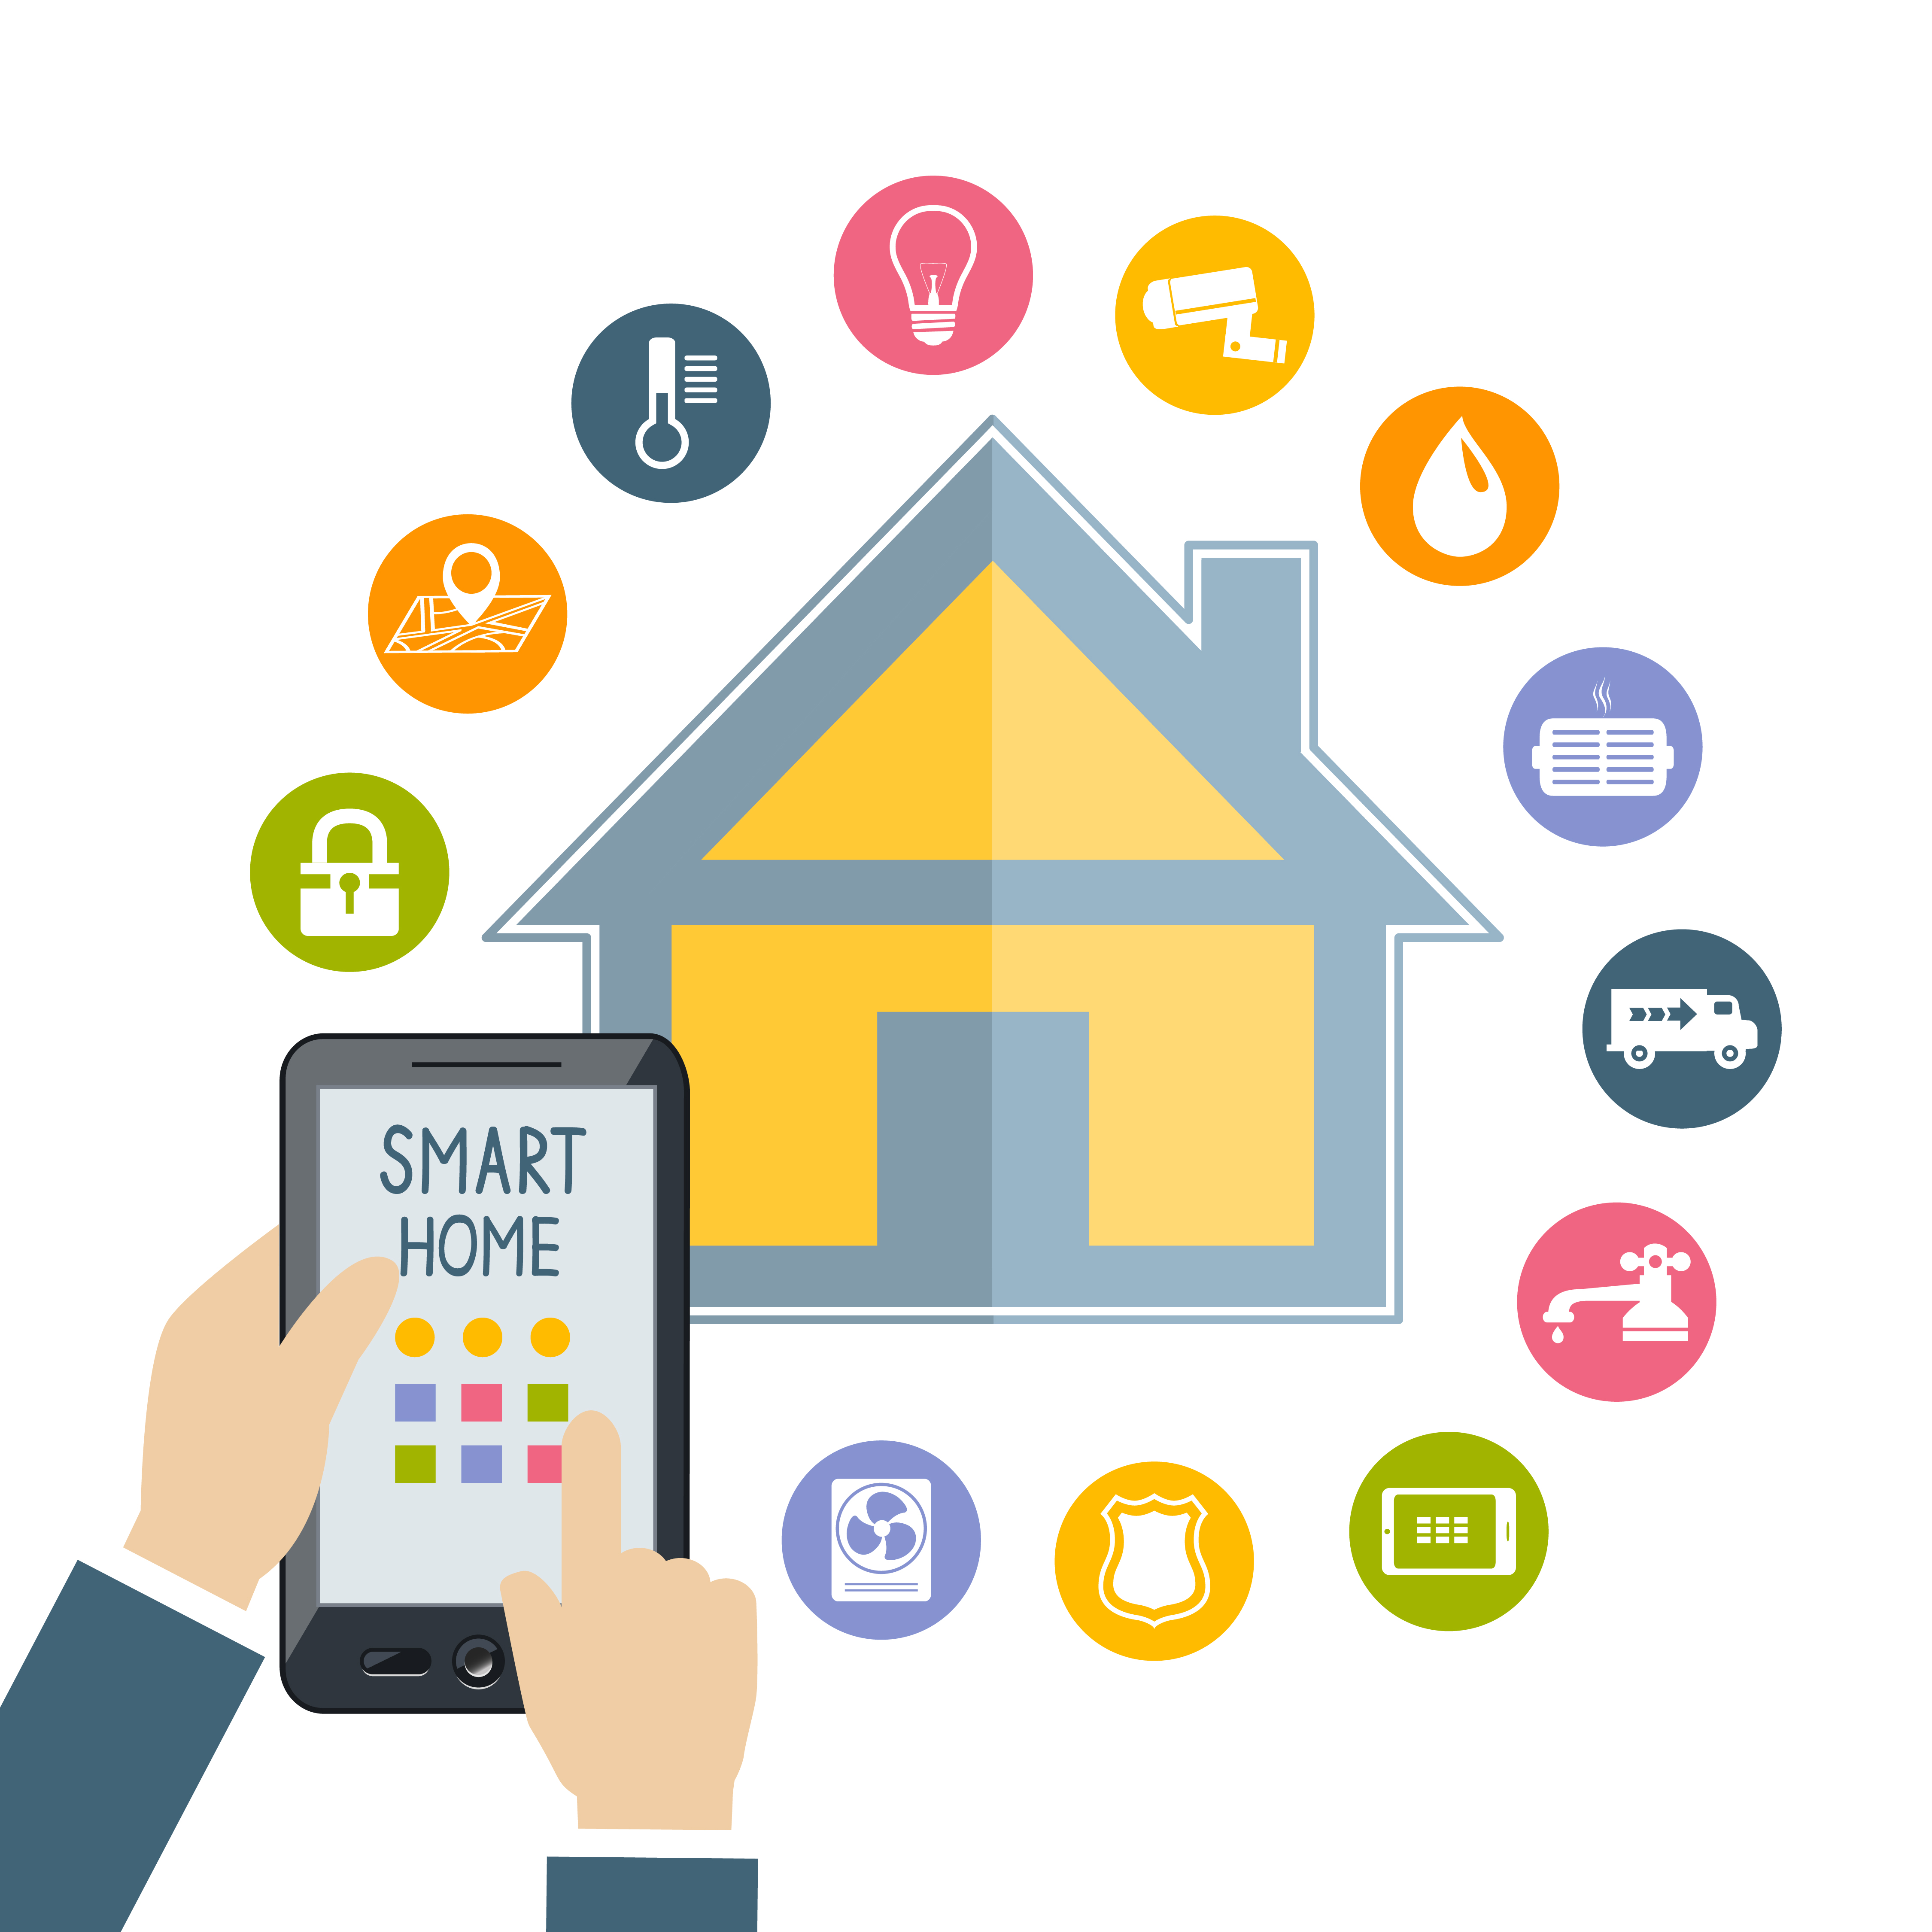
\includegraphics[width=10cm]{Images/Description/smarthome.jpg}
\caption{Smart home}
\end{figure}

\subsection{Mục tiêu và phạm vi dự án}

\indent Mục tiêu chính của nghiên cứu là phát triển một hệ thống điều khiển linh hoạt và hiệu quả, cho phép người dùng tương tác với các thiết bị trong nhà bằng cách sử dụng cử chỉ tự nhiên của bàn tay. Thay vì phải dựa vào ứng dụng di động hoặc giọng nói, người dùng có thể dễ dàng kiểm soát môi trường xung quanh chỉ bằng cách di chuyển bàn tay.

\indent Dự án sẽ tập trung vào việc phát triển và triển khai hệ thống sử dụng cử chỉ bàn tay và kết hợp cảm biến flex để thu thập dữ liệu. Nghiên cứu không chỉ giới thiệu một cách mới để tương tác với thiết bị, mà còn tập trung vào khả năng linh hoạt và tích hợp của hệ thống.

\subsection{Ý nghĩa thực tiễn}

\indent Nghiên cứu này mang lại ý nghĩa thiết thực bằng cách cải thiện trải nghiệm người dùng trong việc quản lý và điều khiển Smart Home. Kết hợp giữa cử chỉ bàn tay tự nhiên và cảm biến flex không chỉ mang lại sự thuận tiện mà còn tạo ra một phương tiện tương tác mới, giúp người dùng tận hưởng một cách tiếp cận độc đáo và linh hoạt hơn. Đồng thời, việc tích hợp này cũng thúc đẩy sự phát triển của công nghệ Smart Home và đóng góp vào xu hướng thông minh hóa trong cuộc sống hàng ngày.

\begin{figure}[H]
    \centering
    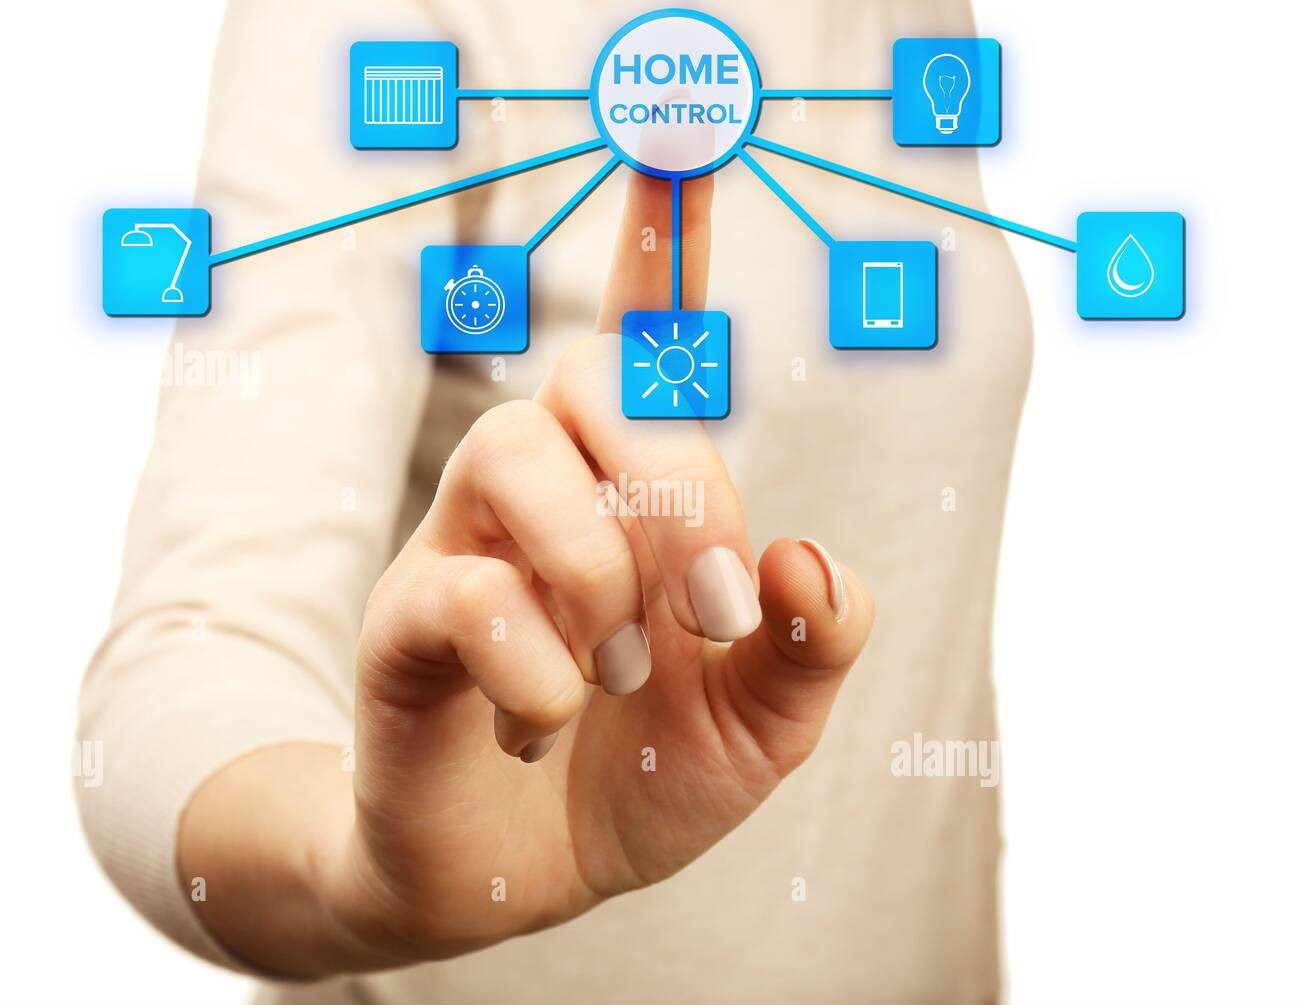
\includegraphics[width=12cm]{Images/Description/smarthome control.jpg}
\caption{Điều khiển bằng cử chỉ}
\end{figure}




